% Evangelos 2009/12/19

\subsection{\label{s:mfReqb}A slice at \reqv}

As became clear in \refsect{sec:mf}, the use of a coordinate \slice\ \refeq{eq:CLEsliceSO2} 
allowed explicit determination of the moving frame map \refeq{eq:CLEmf} and straightforward 
determination of invariant variables \refeq{eq:invLaser}. 
On the other hand \slice\ \refeq{eq:CLEsliceSO2} is defined to be orthogonal
to the group tangent of \SOn{2} restricted in the $x$-irreducible subspace of \SOn{2} 
and this introduces singularities in the transformations \refeq{eq:invLaser}.
Here we will remove this restriction to a coordinate \slice\ and therefore to 
an irreducible subspace and construct a moving frame by defining the slice to be orthogonal 
to the group orbit at a given point in space $\slicep$. The price to pay is that it 
won't be convenient to explicitly write out the transformations to invariant variables
as we did in \refsect{sec:mf}; we will instead implement the moving frame map numerically,
mapping computed trajectories to the \slice.

Specifically, we define a slice by
\beq
(\sspRed - \slicep ) \cdot \sliceTan_a =0
    \,,\qquad
\sliceTan_a  = \Lg_a \, \slicep
\,.
\ee{PCsectQ}
A generic point $\slicep $ not in an invariant subspace (on
the \CLe\ $z$ axis, for example) should suffice to fix a good
\slice. In our \CLe\ example we will choose a point on \reqv\ group orbit,
 $\slicep  = \ssp_{\REQB{1}}$.

As $\slicep  \cdot \sliceTan_a =0$ by the antisymmetry of
$\Lg_a$, the slice condition \refeq{PCsectQ} determines
$\theta$ for a given $\ssp$ by
\beq
0 = \sspRed \cdot \Lg_a \, \slicep
  %= \LieEl(\theta) \cdot \hat{\ssp}   \cdot \Lg \cdot \slicep
	=\ssp \cdot \LieElrep(\theta)^T \Lg_a \, \slicep
\,.
\ee{PCsectQ1}



%%%%%%%%%%%%%%%%%%%%%%%%%%%%%%%%%%%%%%%%%%%%%%%%%%%%%%%%%%%%%%%%
%computed with vaggelis/testing/flows/CLEfinalTmp.nb
\begin{figure}[ht]
\begin{center}
  (\textit{a})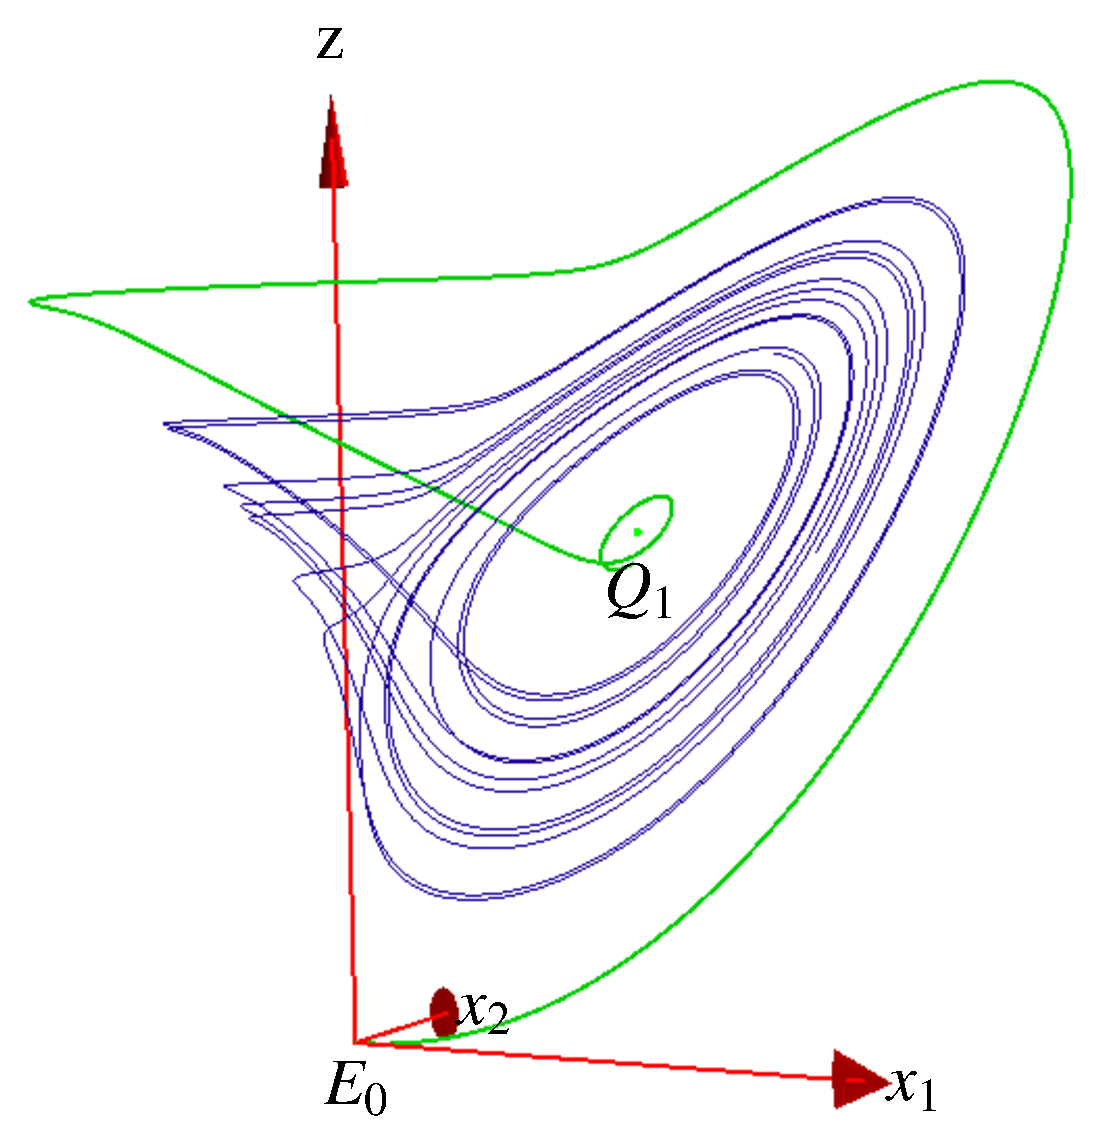
\includegraphics[width=0.35\textwidth]{../figs/CLEmfReqb1}
~~~~(\textit{b})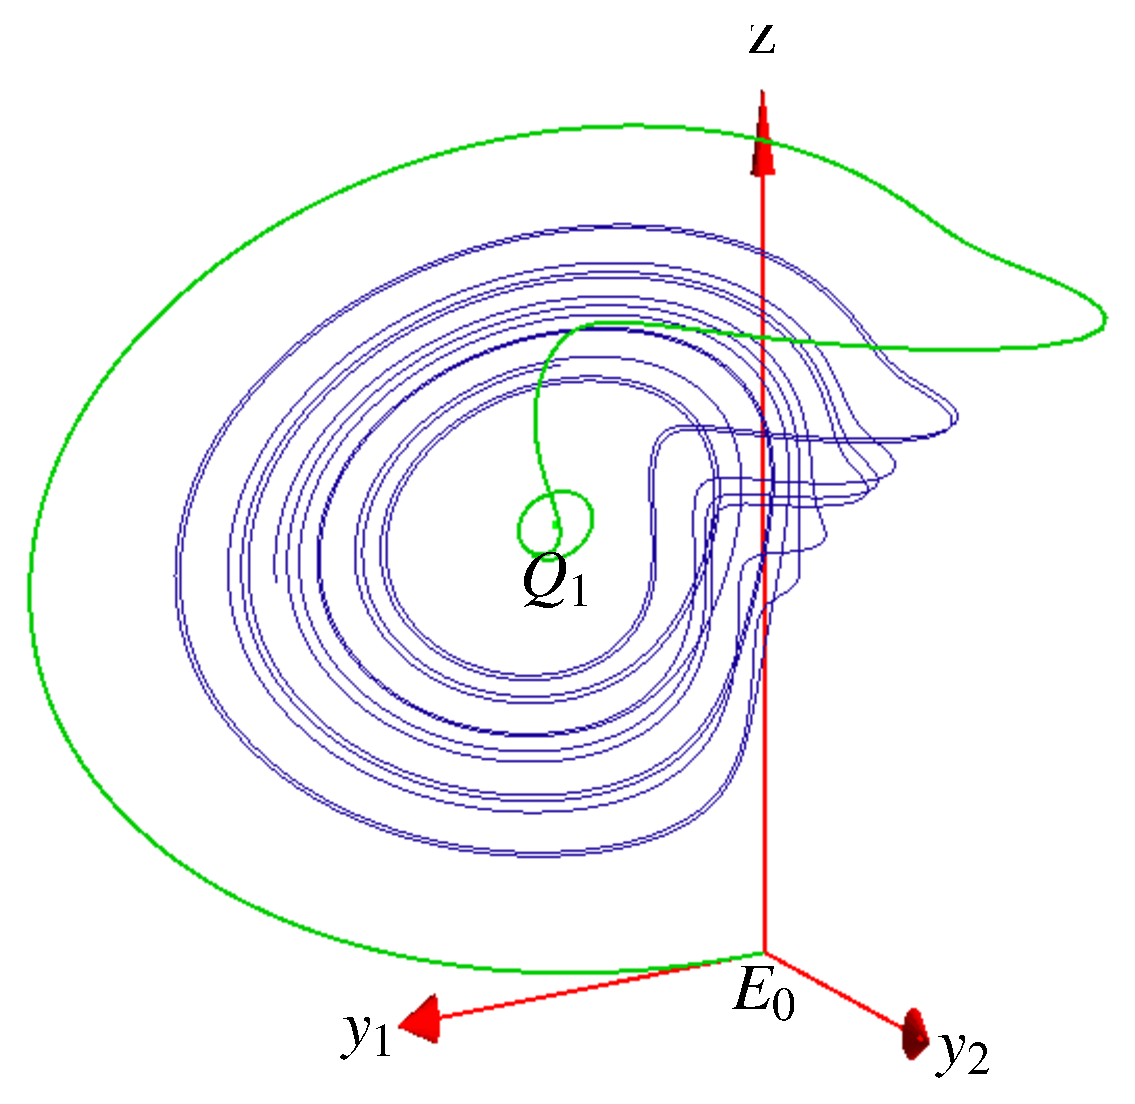
\includegraphics[width=0.35\textwidth]{../figs/CLEmfReqb}
\end{center}
\caption{ \Statesp\
portraits of \CLe\ dynamics for $e=1/10$, $\ImrCLor=0$
in \reducedsp. We use a slice defined by \refeq{PCsectQ1} with  $\slicep  = \ssp_{\REQB{1}}$.
    }
\label{fig:CLEmfReqb1}
\end{figure}
%%%%%%%%%%%%%%%%%%%%%%%%%%%%%%%%%%%%%%%%%%%%%%%%%%%%%%%%%%%%%%%%


  